\documentclass{article}
\usepackage[utf8]{inputenc}
\usepackage{multicol}
\usepackage{amsmath}
\usepackage{float}
\usepackage{epsfig,graphicx}
\usepackage{xcolor,import}
\usepackage{caption}
\usepackage{subcaption}
\usepackage[font=small,labelfont=bf]{caption}
\usepackage{siunitx}
\usepackage[german]{babel}
\usepackage{textcomp}
\usepackage{mathtools}
\usepackage{subcaption}
\usepackage{cleveref}

\begin{document}


\thispagestyle{empty}
			\begin{center}
			\Large{Fakultät für Physik}\\
			\end{center}
\begin{verbatim}


\end{verbatim}
							%Eintrag des Wintersemesters
			\begin{center}
			\textbf{\LARGE SOMMERSEMESTER 2015}
			\end{center}
\begin{verbatim}


\end{verbatim}
			\begin{center}
			\textbf{\LARGE{Physikalisches Praktikum II}}
			\end{center}
\begin{verbatim}




\end{verbatim}

			\begin{center}
			\textbf{\LARGE{PROTOKOLL}}
			\end{center}
			
\begin{verbatim}





\end{verbatim}

			\begin{flushleft}
			\textbf{\Large{Experiment (Nr., Titel):}}\\
							%Experiment Nr. und Titel statt den Punkten eintragen
			\LARGE{}	
			\end{flushleft}

\begin{verbatim}

\end{verbatim}	
							%Eintragen des Abgabedatums, oder des Erstelldatums des Protokolls
			\begin{flushleft}
			\textbf{\Large{Datum:}} \Large{}
			\end{flushleft}
			
\begin{verbatim}
\end{verbatim}
							%Namen der Protokollschreiber
		\begin{flushleft}
			\textbf{\Large{Bachleitner Veronika, Grafendorfer Erik}} 
			\end{flushleft}

\begin{verbatim}


\end{verbatim}
							%Kurstag und Gruppennummer, zb. Fr/5
			\begin{flushleft}
			\textbf{\Large{Kurstag/Gruppe:}} \Large{FR/1}
			\end{flushleft}

\begin{verbatim}






\end{verbatim}
							%Name des Betreuers, das Praktikum betreute.
			\begin{flushleft}
			\LARGE{\textbf{Betreuer:\Large{ }}}		
			\end{flushleft}
			
\section{Aufgabenstellung}

\section{Theorie}
\subsection{Auflösungsvermögen eines Gitters}

Bei der Beugung an einem Gitter gibt es folgende wichtige Größen:\\
\\
\begin{tabular}{|c|c|}
\hline
N & Anzahl der Spalte\\
B & Breite der Spaltblende\\
b & Spaltbreite\\
a & Spaltabstand\\
\hline
\end{tabular}
\vspace{0.5cm}
\\
Es gibt zwei verschiedene Aspekte, die dann passieren. Erstens die Beugung am Einzelspalt. Zweitens kommt zusätzlich noch Interferenz dazu, die durch die an den einzelnen Spalten abgebeugten Lichtstrahlen entsteht. Daher kommt es bei der Beugung am Gitter auf dem Schirm zu einem Interferenzbild: Treffen jeweils die Maxima und Minima der kohärenten Lichtwellen aufeinander kommt es zu konstruktiver Interferenz. Sind die Maxima und Minima jedoch zueinander verschoben kommt es zu destruktiver Interferenz (vollkommen destruktiv, wenn dazwischen der Abstand einer halben Wellenlänge liegt).\\
Man kann also am Schirm mehrere Interferenzmaxima beobachten. Da die Intensität der sekundären Maxima umgekehrt proportional zur Anzahl der Spalte zum Quadrat ist, nimmt sie mit höherer Spaltanzahl auch schnell ab.\\
Gibt es zwei benachbarte Wellenlängen $\lambda$ und $\lambda+\Delta\lambda$ können diese nicht immer getrennt beobachtet werden. Dazu müssen sich die unterschiedlichen Ablenkwinkel der Intensitätsmaxima mindestens um eine volle Halbwertsbreite unterscheiden. Ob die benachbarten Wellenlängen beobachtbar sind kommt auf das \textit{spektrale Auflösungsvermögen} des Gitters an.\\
Das spektrale Auflösungsvermögen ist abhängig von der Ordnung $n$ und der wirksamen Strichzahl $N$. Es kann berechnet werden mittels:
$$A=\frac{\lambda}{\Delta\lambda}=n\cdot N$$
\\
Alle weitere Berechnungen sind der Sparte \textit{Ergebnisse} zu entnehmen, da dies Teil der Aufgabe war und somit im \textit{Theorie}-Abschnitt schon vorgegriffen wäre.


\subsection{}

\subsection{Michelson-Interferometer}

Das Michelson-Interferometer nutzt die Interferenz zwischen kohärenten Wellenzügen um die Unterschiede zweier Wege zu messen. Das bedeutet, dass kohärentes Laserlicht an einem Beamsplitter auf zwei Wege geschickt wird, um an deren Ende reflektiert, wieder vereint und dabei zur Interferenz gebracht zu werden. Das Interferenzmuster lässt sich auf einem Schirm beobachten - es entsteht durch einen Phasenunterschied der beiden Lichtwellen. Dieser Unterschied kann auf verschiedene Arten erzeugt werden, zum Beispiel durch unterschiedlich lange Wege, unterschiedliche optische Beschaffenheit der Medien, durch die die Lichtwellen ziehen, oder auch durch Bewegung der Apparatur, ein Effekt, der beispielsweise beim Laserkreisel in Flugzeugen Anwendung findet :)\\
Im vorliegenden Experiment wird durch eine bekannte Änderung der Länge eines der Wege $\Delta l$ das Interferenzmuster verändert. Mit der Formel 
\begin{equation}
\label{equ:Michelson}
2\cdot \Delta l= \lambda \cdot N
\end{equation}
lässt sich die Wellenlänge des Lichts bestimmen - wobei N die Anzahl der entstehenden oder verschwindenden Intensitätsmaxima oder -minima bedeutet. 
\section{Aufbau}
\subsection{Auflösungsvermögen eines Gitters}
Wir verwenden eine Quecksilberdampflampe, deren Licht wir auf ein Gitter fallen lassen und durch ein Fernrohr beobachten. Das verwendete Licht hat dabei zwei gelbe Anteile, deren Wellenlängen nah beinander liegen. Wenn wir einen weiten Spalt vor das Gitter stellen und ihn langsam verengen, können wir dabei die Zahl der Gitterstriche verringern, bis das Auflösungsvermögen des Gitters so gering ist dass die beiden gelben Striche zu einem verwischt werden. Darauf warten wir und messen dann die Breite des Spaltes mit einem Kathetometer.
\subsection{Michelson-Interferometer}
Wir verwenden einen Laser, einen Beamsplitter, zwei Spiegel, einen Schirm und viele rechte Winkel um ein Interferenzmuster nach vorher beschriebener Methode zu erzeugen. Dann wird einer der Spiegel mittels einer Mikrometerschraube mit einer Schraubenkonstante von 0.5$\mu$m verschoben und die dabei auftauchenden Intensitätsminima gezählt. 
\section{Durchführung}
\subsection{Auflösungsvermögen eines Gitters}
Wir messen die Breite des Spaltes beim Verwischen der beiden gelben Linien für drei Beugungsordnungen links und rechts der Mitte. Die Unsicherheit der Breite des Spaltes kann mit $\pm$0.01 mm angegeben werden, allerdings ist der genaue Moment des Verwischens der Linien mit freiem Auge gemessen und die Messung damit einer weiteren Unsicherheit unterworfen, die wir hier allerdings nicht betrachten.
\subsection{Michelson-Interferometer}
Es werden drei mal 100 Minima gezählt.\\
Das Interferometer war bereits aufgebaut und gut justiert, darum konnten wir die Messung sogleich durchführen.\\
Aufgrund der anstrengenden Messmethode und unserer müden Augen müssen wir annehmen, dass N eine Unsicherheit hat: $N=(100 \pm 5)$.

\section{Ergebnisse}
\subsection*{Auflösungsvermögen eines Gitter}
% ! Unsicherheiten der Einzelwerte von a fehlen noch
%
%
%Berechnen Sie das Auflösungsvermögen A aus den Angaben.
Die Wellenlängen der Quecksilber-Linien sind $\lambda=576.96nm$ und $\lambda=579.07nm$.\\
\\
Das Auflösungsvermögen kann berechnet werden mittels:
$$\boxed{A=\frac{\lambda}{\Delta\lambda}=\frac{576.96}{2.11}=273.44}$$
wobei wir für $\Delta\lambda$ die Differenz der beiden Wellenlängen genommen haben.\\
\\
%Leiten Sie die Formel zur Berechnung der Gitterkonstante aus dem Auflösungsvermögen und den Messgrößen her.
Das Auflösungsvermögen ist außerdem gegeben durch $A=n\cdot N$. Über die Formel $B=a\cdot N \Rightarrow N=\frac{B}{a}$ können wir also das Auflösungsvermögen und die Gitterkonstante in Beziehung stellen:
$$A=n\frac{B}{a}$$
Formen wir um, können wir aus den gemessenen Spaltbreiten zur jeweiligen Ordnung die Gitterkonstante berechnen:
$$\boxed{a=n\frac{B}{A}}$$
\\
Wir kommen nun zum experimentellen Teil und messen die Spaltbreite, bei denen die beiden Wellenlängen gerade nicht mehr zu unterscheiden sind. Das führen wir für 3 Ordnungen rechts und links des Zentralbildes durch.
%Bestimmen Sie die Gitterkonstante und geben Sie diese mit Fehler an.
\begin{table}[H]
\begin{center}
\begin{tabular}{|r|l|l|}
\hline
n & B (mm, $\pm 0.01$) & a (mm)\\
\hline
R1 & 5.11 & 0.019\\
R2 & 1.85 & 0.013\\
R3 & 1.02 & 0.011\\
L1 & 5.15 & 0.019\\
L2 & 2.29 & 0.017\\
L3 & 1.78 & 0.019\\
\hline
%\caption{Spaltbreiten zu den jeweiligen Ordnungen. R: Rechts, L: Links.}
\end{tabular}
\caption{Spaltbreiten zu den jeweiligen Ordnungen und daraus berechnete Gitterkonstante. R: Rechts, L: Links.}
\end{center}
\end{table}
\vspace{0.3mm}
Aus den jeweils berechneten Werten für die Gitterkonstante $a$ berechnen wir einen Mittelwert mit Standardabweichung:
$$\boxed{\bar{a}=(0.016 \pm 0.004)mm}$$

\subsection{Spektrometrie}

\begin{figure}[H]
\centering
\begin{subfigure}[h]{0.4\textwidth}
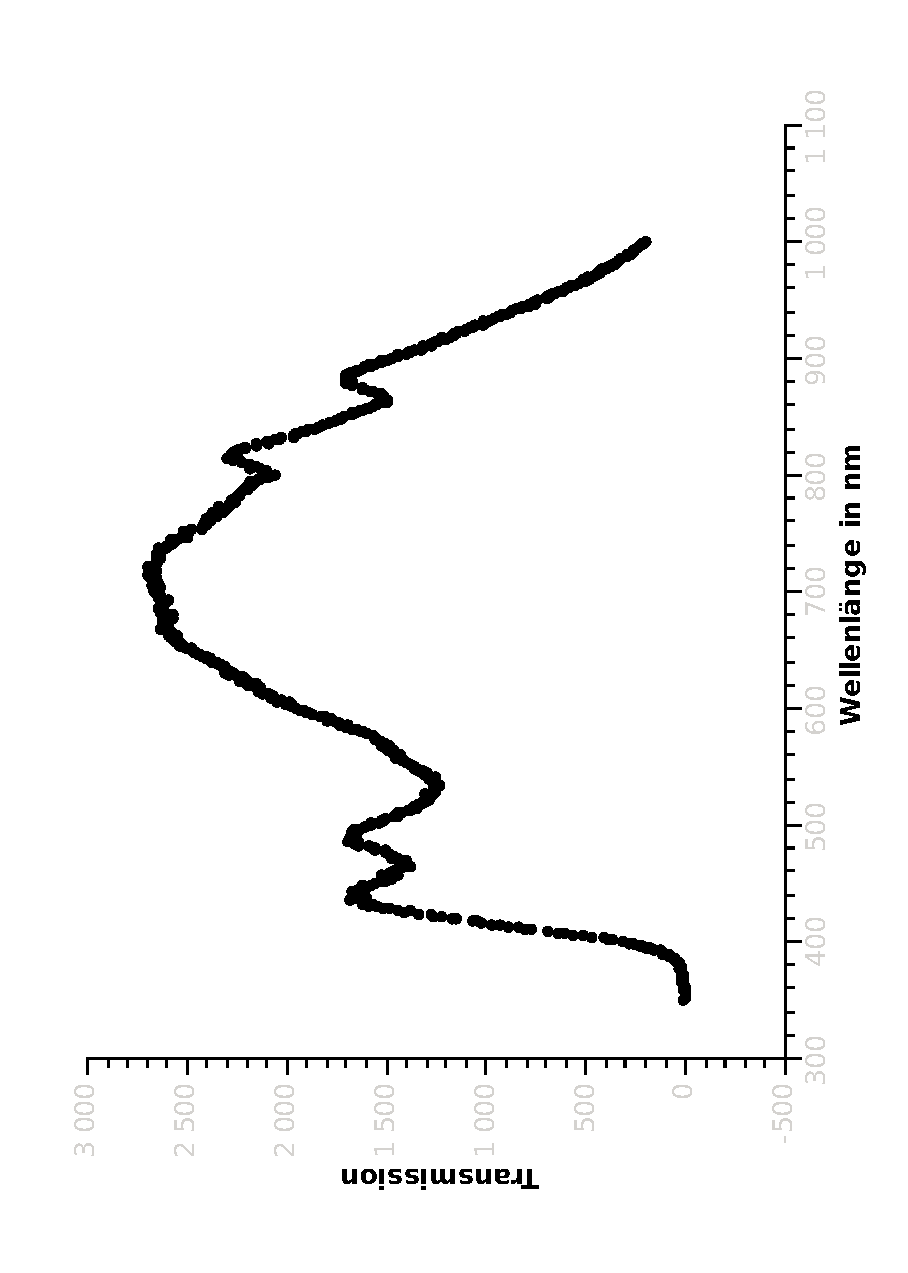
\includegraphics[width=\textwidth ,angle=-90]{eps/referenztrans1.eps}
\caption{Referenzspektrum mit leerem Probenbehälter}
\end{subfigure}
\begin{subfigure}[h]{0.4\textwidth}
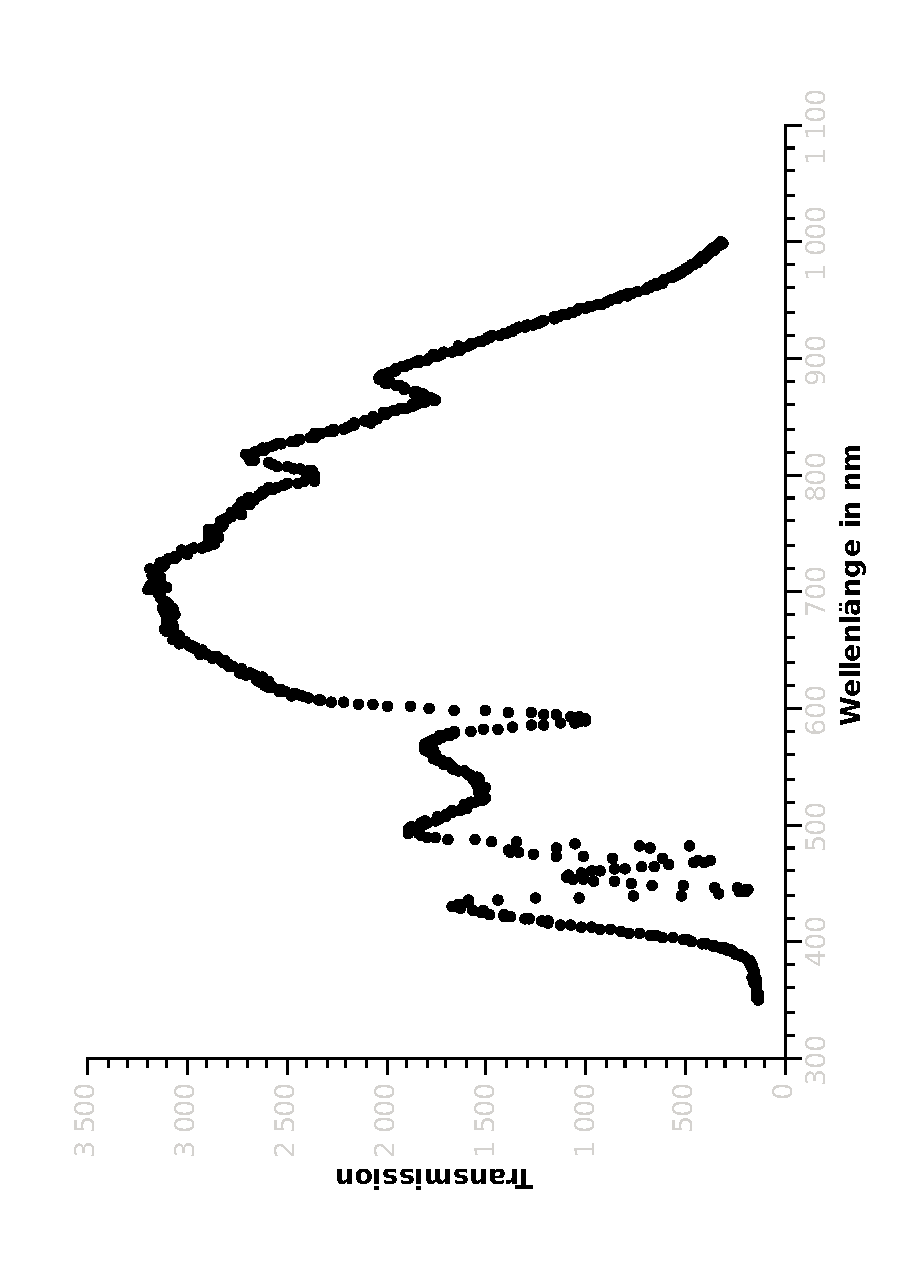
\includegraphics[width=\textwidth ,angle=-90]{eps/probeAtrans.eps}
\caption{Transmissionsspektrum von Probe A}
\end{subfigure}
\end{figure}


\begin{figure}[H]
\centering
\begin{subfigure}[h]{0.4\textwidth}
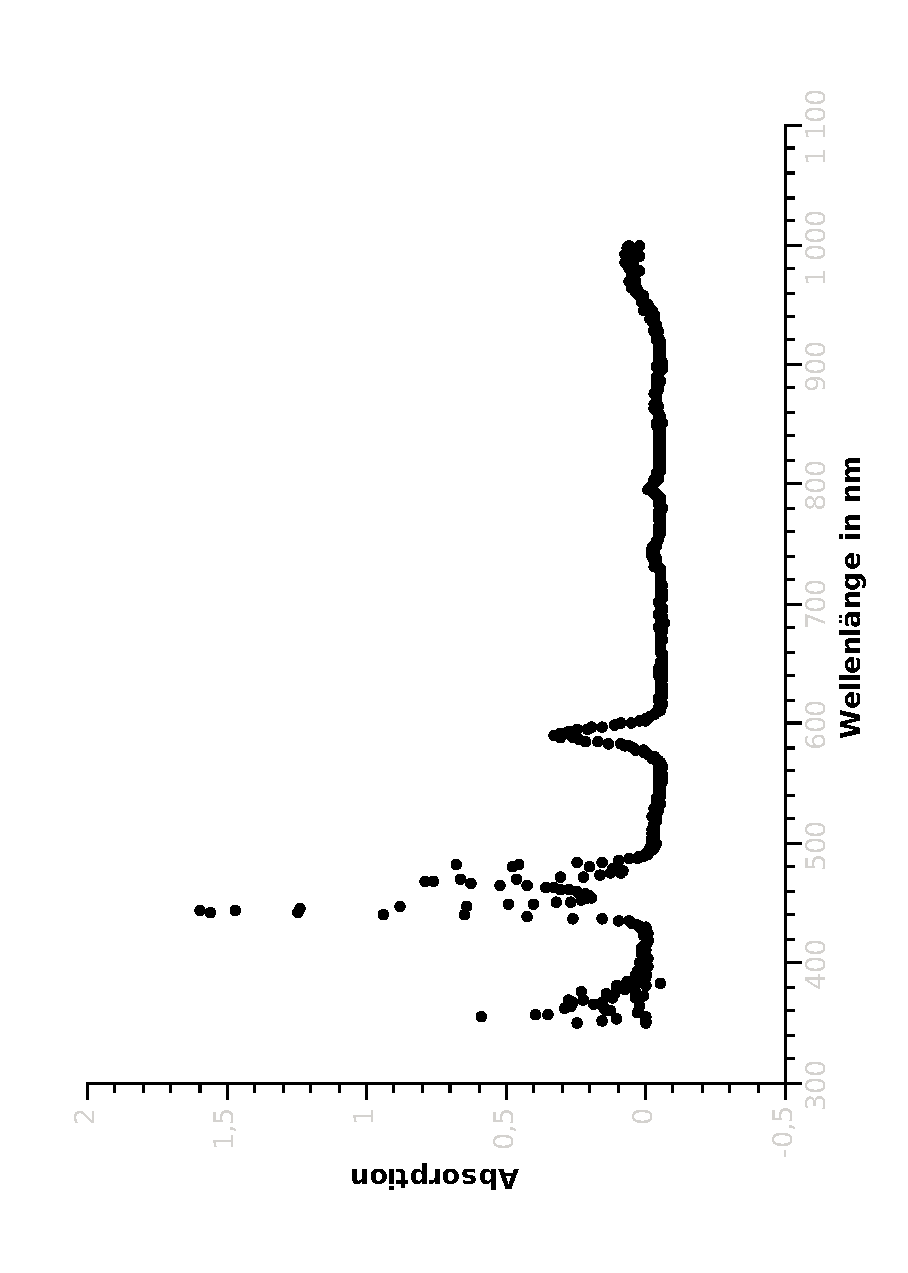
\includegraphics[width=\textwidth ,angle=-90]{eps/probeAabs.eps}
\caption{Absorptionsspektrum \\ von Probe A}
\end{subfigure}
\begin{subfigure}[h]{0.4\textwidth}
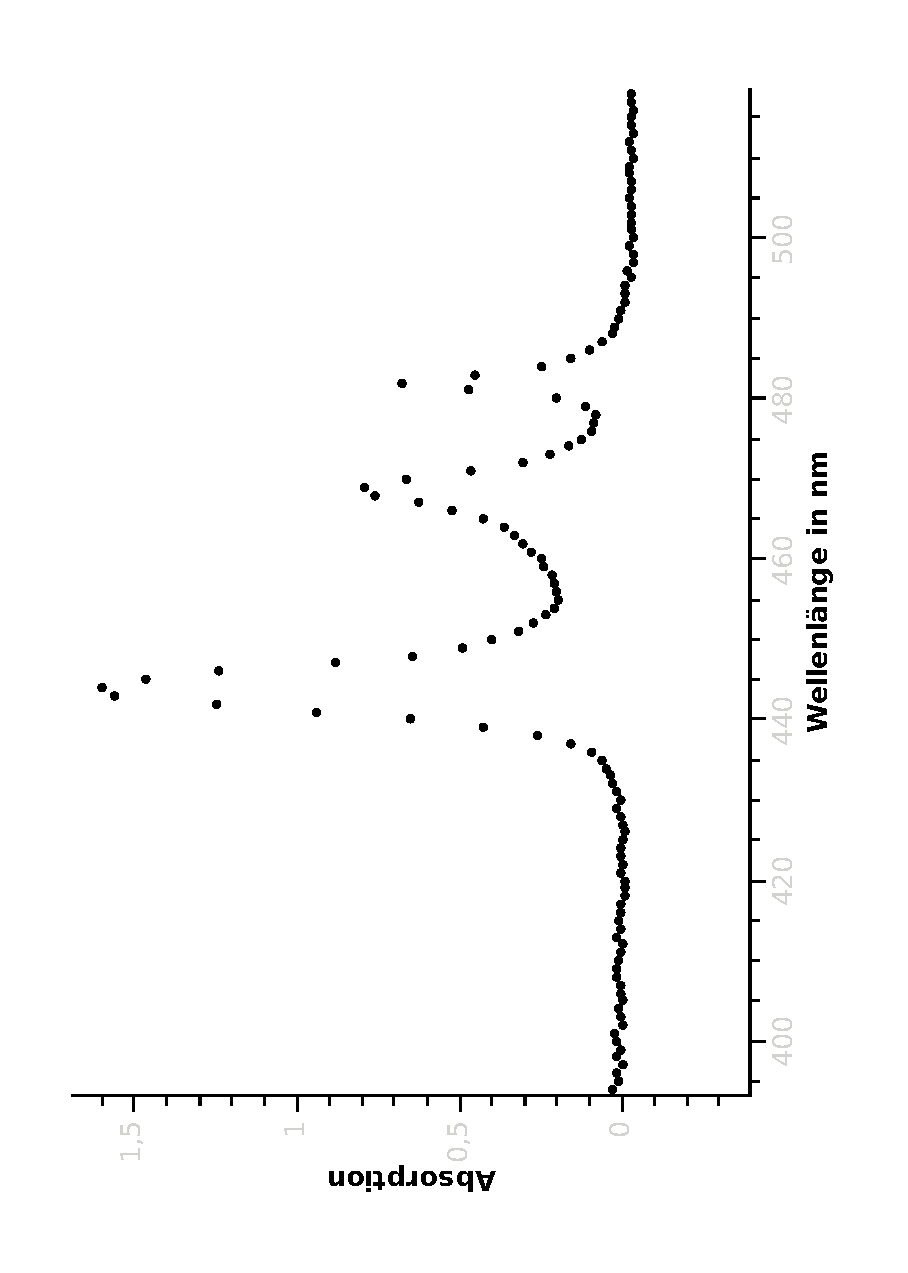
\includegraphics[width=\textwidth ,angle=-90]{eps/probeAabsdetail.eps}
\caption{Detail des selben Spektrums}
\end{subfigure}
\end{figure}

\begin{table}[H]
\centering
\caption{Absorption der Probe A}
\label{AbsProbeA}
\begin{tabular}{|c|c|} \hline
Wellenlänge [nm] & Absorption  \\ 
\hline 444 & 1.6 \\
469 & 0.8 \\
482 & 0.7 \\
590 & 0.3 \\
\hline
\end{tabular}
\end{table}


\begin{figure}[H]
\caption{Messungen \label{fig:gluehlampen} mit der Glühlampe}

\centering
\begin{subfigure}[h]{0.4\textwidth}
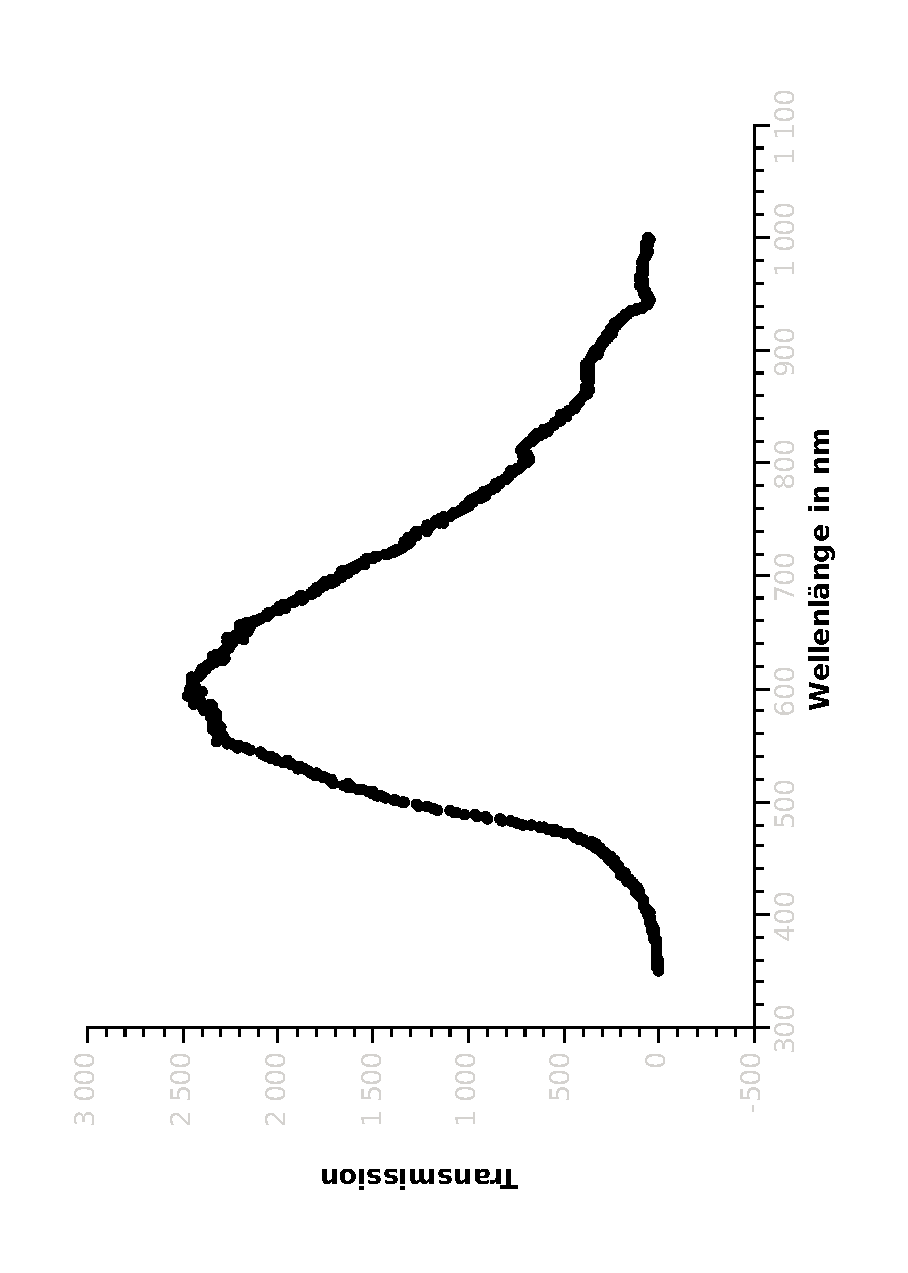
\includegraphics[width=\textwidth ,angle=-90]{eps/leerproberef.eps}
\caption{Referenzspektrum der Glühlampe}
\end{subfigure}
\begin{subfigure}[h]{0.4\textwidth}
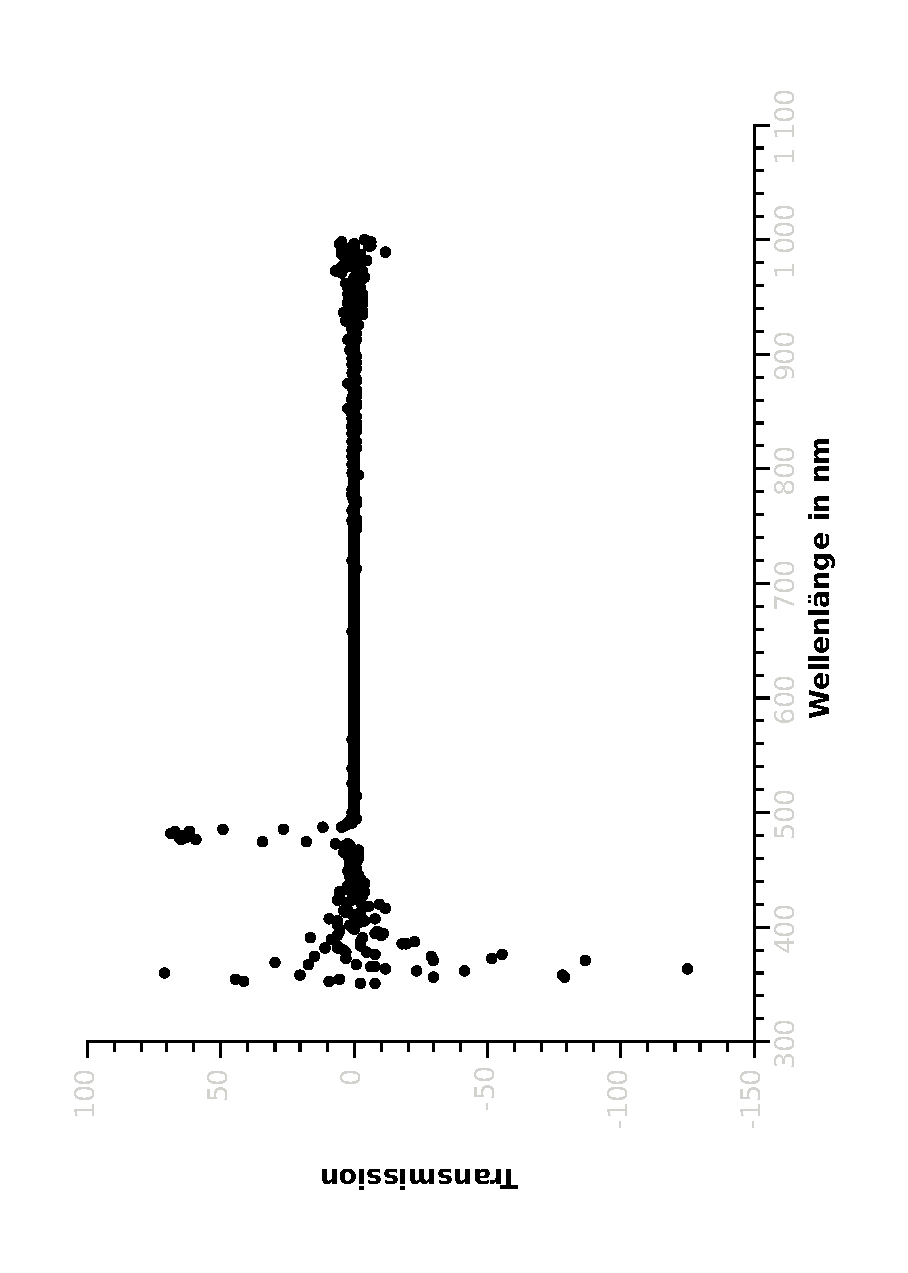
\includegraphics[width=\textwidth ,angle=-90]{eps/intertranswhole.eps}
\caption{Transmissionsspektrum des Interferenzfilters}
\end{subfigure}
\begin{subfigure}[h]{0.4\textwidth}

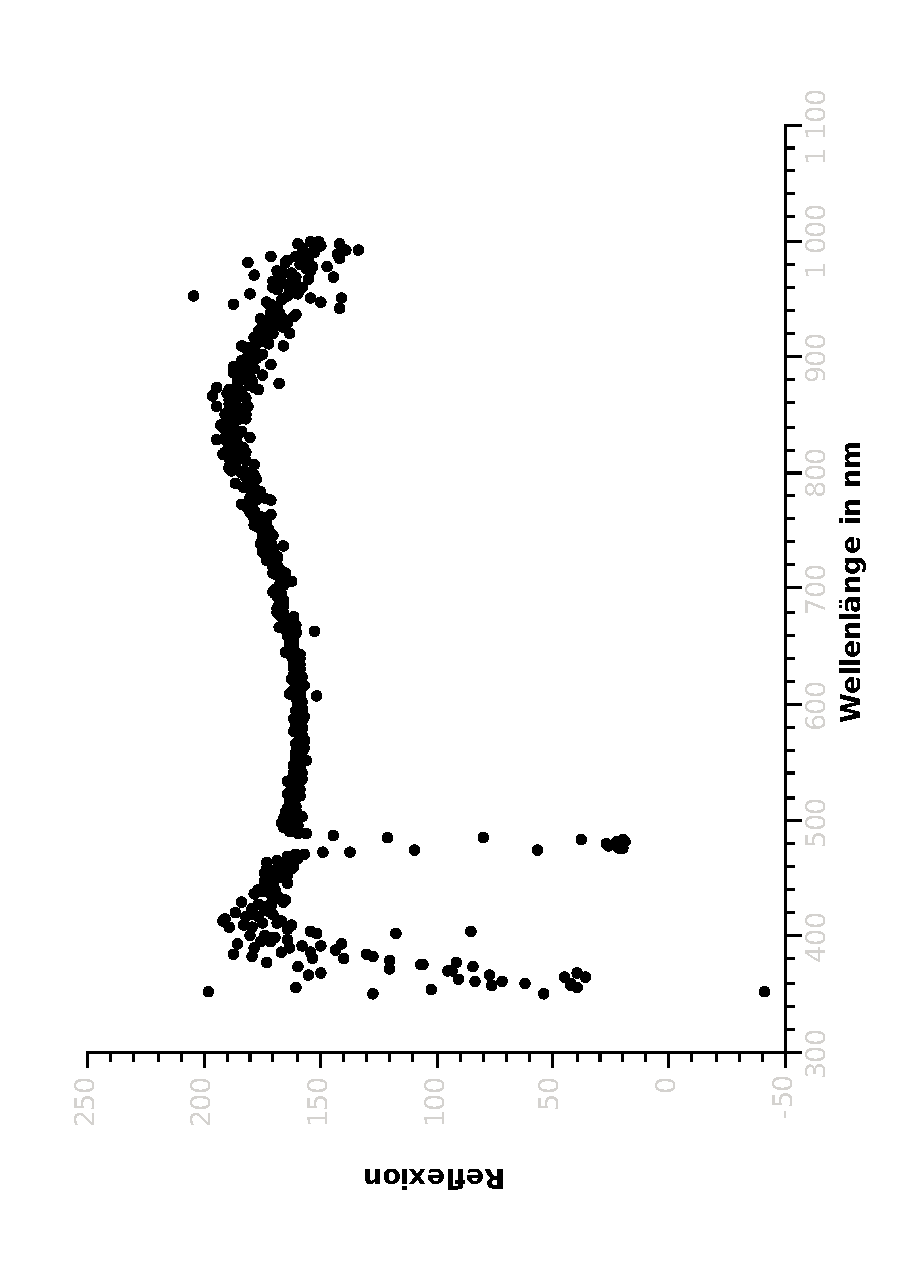
\includegraphics[width=\textwidth ,angle=-90]{eps/interreflsilber.eps}
\caption{Reflexionsspektrum der \label{fig:silverrefl} silbernen Seite des Interferenzfilters}
\end{subfigure}
\begin{subfigure}[h]{0.4\textwidth}
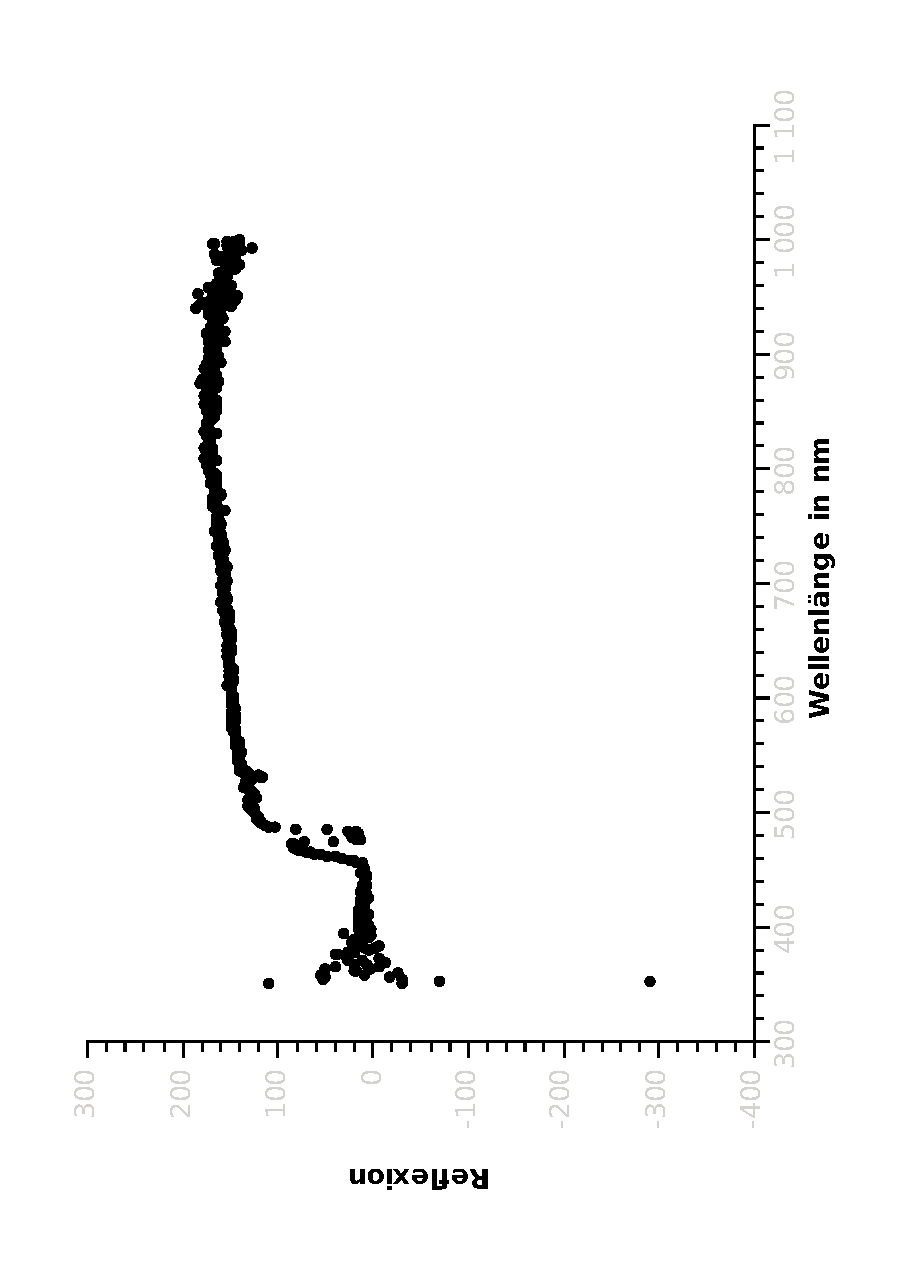
\includegraphics[width=\textwidth ,angle=-90]{eps/interreflgruen.eps}
\caption{Reflexionsspektrum \label{fig:greenrefl} der grünen Seite des Interferenzfilters}
\end{subfigure}
\begin{subfigure}[h]{0.4\textwidth}
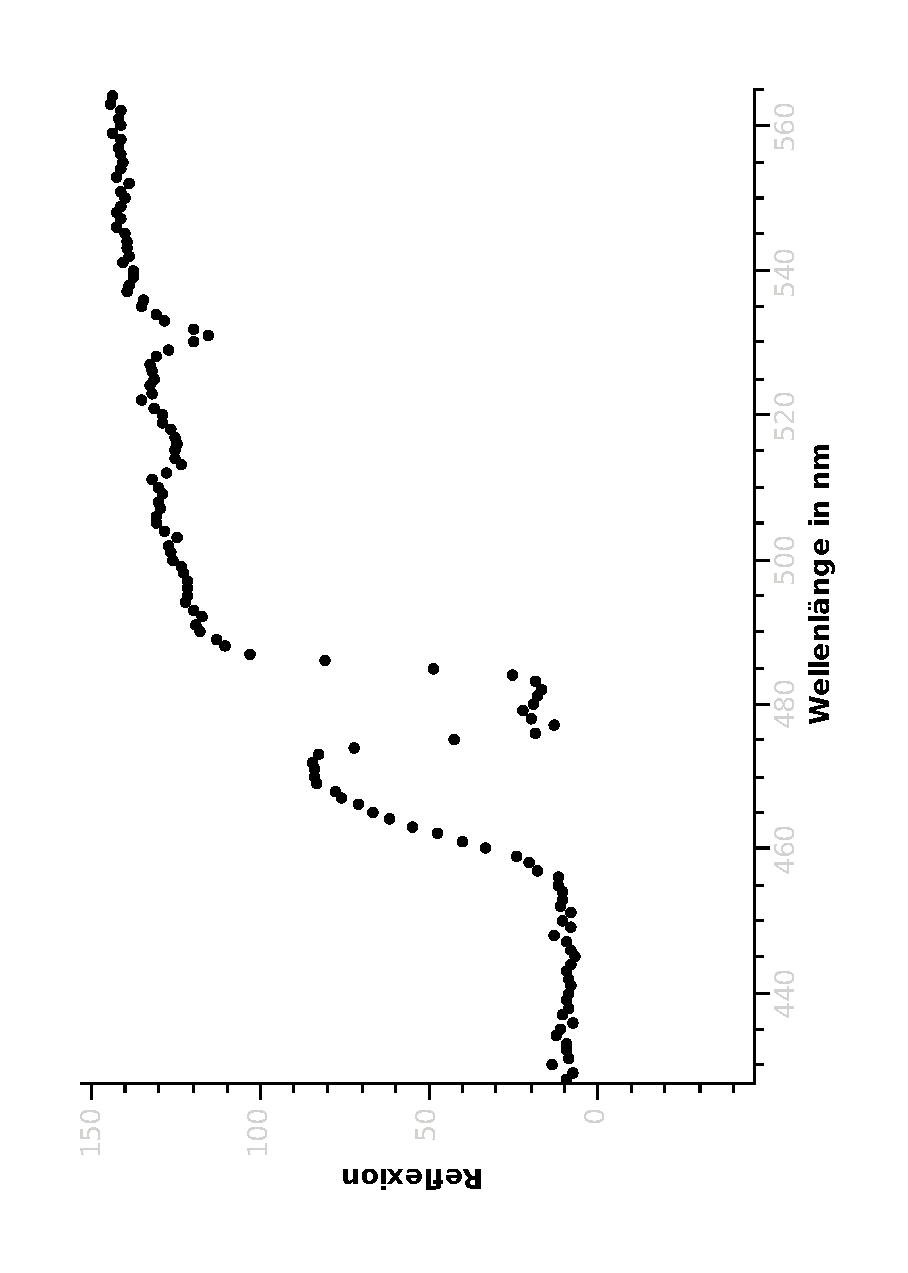
\includegraphics[width=\textwidth ,angle=-90]{eps/interrefldetail.eps}
\caption{Detail des Reflexionsspektrums der grünen Seite des Interferenzfilters}
\end{subfigure}
\end{figure}

\begin{figure}
\centering
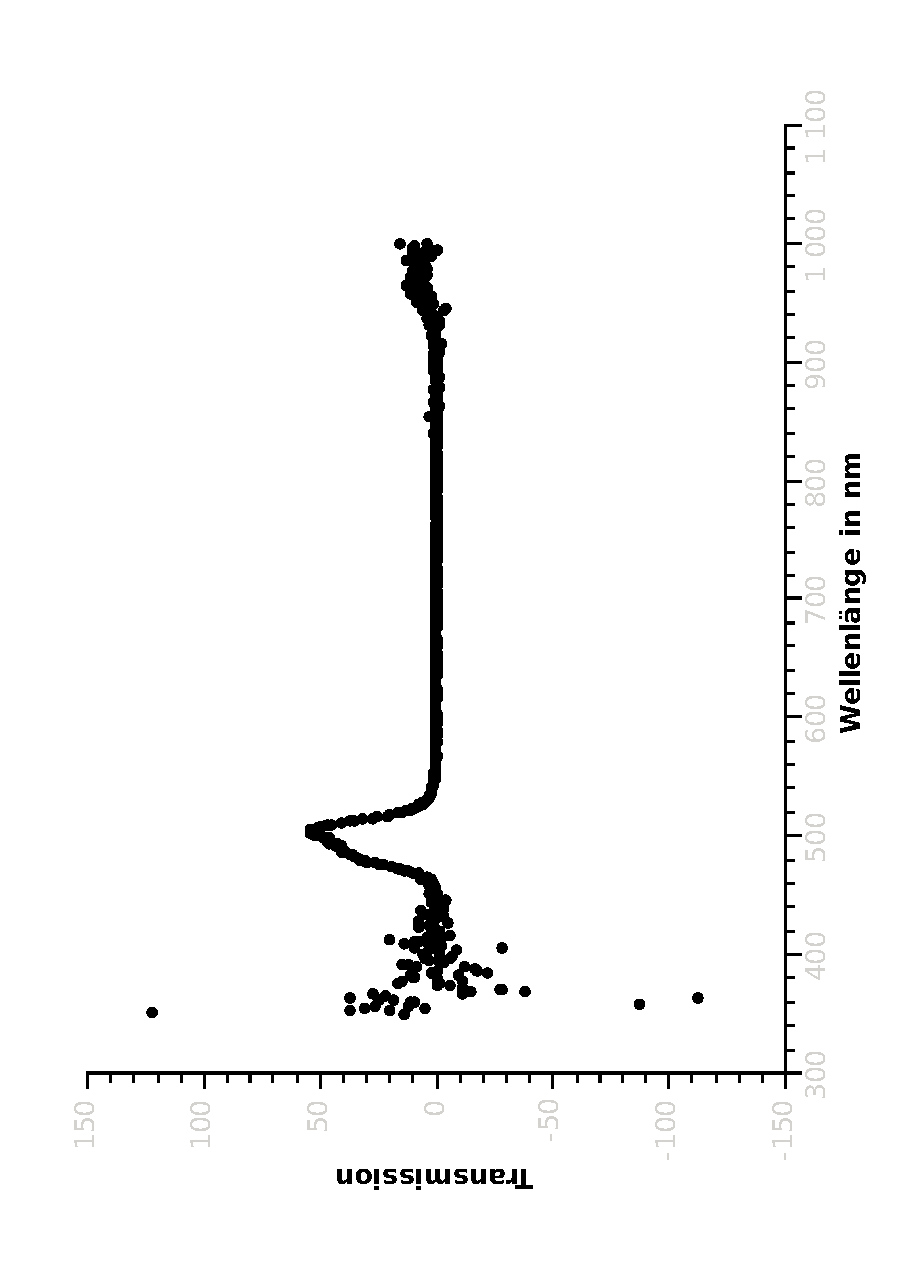
\includegraphics[width=0.4\textwidth, angle=-90]{eps/glasfilterk3.eps}
\caption{Transmissionsspektrum des gelbgrünen Glasfilters K3}
\end{figure}

Die Bandbreite der Transmission, das FWHM, des Interferenzfilters wurde mit dem Fit einer Gaußschen Glockenkurve in qtiplot berechnet, und zwar zu:
\begin{center}
\fbox{(8.3 $\pm$ 0.4)nm}
\end{center}
um eine Wellenlänge von \fbox{(480 $\pm$ 1) nm}.\\

Bei den Reflexionsspektren des Interferenzfilters \subref{fig:silverrefl} fällt auf, dass bei der silbrigen Seite ein großer Teil des Lichts reflektiert wird, nur eine kleine Bandbreite im Bereich von 480nm fehlt - was in den grünen Bereich des sichtbaren Lichts fällt. Laut wikipedia ist Licht von 480 bis 560 nm grün. Also sollte die silbrige Seite leicht rot oder orange getüncht erschienen sein - in der Komplementärfarbe der entsprechenden grünen Bandbreite - woran wir uns aber nicht sicher erinnern können. \\
Beim Reflexionsspektrum der grünen Seite  \subref{fig:greenrefl} sieht man schön dass die Wellenlängen unter 460 nm kaum reflektiert werden - es gibt wieder ein Minimum bei 480nm - und darüber aber wieder stärker. Die fehlenden Wellenlängen lassen den Filter jedenfalls grün erscheinen.
\subsection{Michelson-Interferometer}
\begin{table}[H]
\begin{center}
\begin{tabular}{c}
$(29.5\pm 0.5)\mu m$\\
$(32.5\pm 0.5)\mu m$\\
$(32.0\pm 0.5)\mu m$\\
\end{tabular}
\caption{Spiegelverschiebung $l$ für $N=100 \pm 5$ Umdrehungen}
\end{center}
\end{table}
\vspace{0.3mm}

Mit der Formel $2 l=\lambda N$ können wir die Wellenlänge des Lasers berechnen:
%Wir verwenden hier $l$ statt $\Delta l$ für die Spiegelverschiebung, da sie ansonsten mit der Unsicherheit der Verschiebung (die wir $\Delta l$ nennen) verwechselt werden könnte.\\
%Die Wellenlänge wird also berechnet mittels
$$\lambda=\frac{2l}{N}$$
\\
Wir führen hier eine komplette Fehlerrechnung durch:
$\Delta l$ und $N$ haben jeweils eine Unsicherheit, die in der Gaußschen Fehlerfortpflanzung verwendet werden müssen.\\
$$\Delta \lambda=\sqrt{\left(\frac{\Delta l}{l}\right)^2+\left(\frac{\Delta N}{N}\right)^2}=\sqrt{\left(\frac{0.5}{l}\right)^2+\left(\frac{5}{100}\right)^2}=0.053 \mu m$$
Diese Unsicherheit gilt glücklicherweise für alle drei Werte von $l$.\\
Wir haben nun also: 
\begin{table}[H]
\begin{center}
\begin{tabular}{|c|c|}
\hline
$l$ & $\lambda$\\
\hline
$(29.5\pm 0.5)\mu m$ & $(590 \pm 53)nm$\\
$(32.5\pm 0.5)\mu m$ & $(650 \pm 53)nm$\\
$(32.0\pm 0.5)\mu m$ & $(640 \pm 53)nm$\\
\hline
\end{tabular}
\caption{Spiegelverschiebung und daraus berechnete Wellenlänge}
\end{center}
\end{table}
\vspace{0.3mm}

Der Mittelwert aus diesen drei Werten ist $626nm$ mit der Standardabweichung $32nm$. Da die Unsicherheit der Messwerte größer ist verwenden wir deren Unsicherheit und erhalten das Ergebnis:

$$\boxed{\lambda=(626 \pm 53)nm}$$

\section{Diskussion}
\subsection{Auflösungsvermögen eines Gitters}
Die bei den verschiedenen Ordnungen berechneten Werte der Gitterkonstante schwanken stärker als wir uns gewünscht hätten.\\
Das liegt vor allem an der Verwendung des menschlichen Auges als Richtlinie für den Moment, an dem die beiden Wellenlängen-Linien nicht mehr voneinander unterscheidbar sind. Mit einer Messserie zu jeder Ordnung hätte diese Fehlerquelle vermindert werden können. Da allerdings noch weitere Experimente durchzuführen waren, konnten wir uns dafür nicht die Zeit nehmen.\\
Die Werte liegen allerdings trotzdem einigermaßen gut aneinander. Einzig auffallend ist, dass der Mittlwert $\bar{a}=(0.016 \pm 0.004)mm$ mit seiner Standardabweichung nicht den Wert der dritten Ordnung rechts beinhaltet, $0.016$.

\subsection{Spektrometrie}

Aufgrund des Absorptionsspektrums handelt es sich bei Probe A um Praseodym. \\

Bei den Reflexionsspektren des Interferenzfilters in Bild (\ref{fig:silverrefl}) fällt auf, dass bei der silbrigen Seite ein großer Teil des Lichts reflektiert wird, nur eine kleine Bandbreite im Bereich von 480nm fehlt - was in den grünen Bereich des sichtbaren Lichts fällt. Laut wikipedia ist Licht von 480 bis 560 nm grün. Also sollte die silbrige Seite leicht rot oder orange getüncht erschienen sein - in der Komplementärfarbe der entsprechenden grünen Bandbreite - woran wir uns aber nicht sicher erinnern können. \\
Beim Reflexionsspektrum der grünen Seite in Bild (\ref{fig:greenrefl}) sieht man schön dass die Wellenlängen unter 460 nm kaum reflektiert werden - es gibt wieder ein Minimum bei 480nm - und darüber aber wieder stärker. Die fehlenden Wellenlängen lassen den Filter jedenfalls grün erscheinen.
\subsection{Michelson-Interferometer}
Bei der ersten Messung der Spiegelverschiebung mussten wir erst den Rhythmus finden, in dem das Zählen der Maxima leicht fällt. Daher ist es durchaus möglich, dass das Ergebnis für die Wellenlänge besser stimmt, wenn nur zweiter und dritter Messwert verwendet werden. Dadurch würden wir $\lambda=(645 \pm 53)nm$ erhalten.\\
Da der in den Ergebnissen angegebene Wert aber innerhalb der Unsicherheitsgrenzen im richtigen Bereich liegt, haben wir ihn beibehalten.
																								
\end{document}
